\documentclass[sigconf,review,anonymous]{acmart}
% Check the list of approved packages before you add anything else
% otherwise you will have a bad time when you go to submit to taps!
%https://authors.acm.org/proceedings/production-information/accepted-latex-packages
\usepackage{graphicx}
\usepackage{hyperref}
\usepackage{enumitem}

\copyrightyear{2024}
\acmYear{2024}
\setcopyright{acmlicensed}
\acmConference[Conference acronym `XX]{The cool conference}{June 03--05, 2018}{Woodstock, NY}
\acmBooktitle{Conference acronym `XX:The cool conference, June 03--05, 2018, Woodstock, NY}
\acmDOI{XXXXXXX.XXXXXXX}
\acmISBN{978{-}1{-}4503{-}XXXX{-}X/18/06}


\begin{document}
\title{Super Cool Title}

\author{Shane K. Panter}
    \affiliation{%
    \institution{Department of Computer Science}
    \institution{Boise State University}
    \city{Boise}
    \state{Idaho}
    \country{USA}}
    \email{shanepanter@boisestate.edu}

\author{TBD}
    \affiliation{%
    \institution{Department of Computer Science}
    \institution{Boise State University}
    \city{Boise}
    \state{Idaho}
    \country{USA}}
    \email{TBD}

\begin{abstract}
  \textit{\textbf{Context:}}
  \textit{\textbf{Objective:}}
  \textit{\textbf{Method:}}
  \textit{\textbf{Results:}}
  \textit{\textbf{Conclusions:}}
\end{abstract}

%%
%% The code below is generated by the tool at http://dl.acm.org/ccs.cfm.
%% Please copy and paste the code instead of the example below.
%%
\begin{CCSXML}
<ccs2012>
 <concept>
  <concept_id>00000000.0000000.0000000</concept_id>
  <concept_desc>Do Not Use This Code, Generate the Correct Terms for Your Paper</concept_desc>
  <concept_significance>500</concept_significance>
 </concept>
 <concept>
  <concept_id>00000000.00000000.00000000</concept_id>
  <concept_desc>Do Not Use This Code, Generate the Correct Terms for Your Paper</concept_desc>
  <concept_significance>300</concept_significance>
 </concept>
 <concept>
  <concept_id>00000000.00000000.00000000</concept_id>
  <concept_desc>Do Not Use This Code, Generate the Correct Terms for Your Paper</concept_desc>
  <concept_significance>100</concept_significance>
 </concept>
 <concept>
  <concept_id>00000000.00000000.00000000</concept_id>
  <concept_desc>Do Not Use This Code, Generate the Correct Terms for Your Paper</concept_desc>
  <concept_significance>100</concept_significance>
 </concept>
</ccs2012>
\end{CCSXML}

\ccsdesc[500]{Do Not Use This Code~Generate the Correct Terms for Your Paper}
\ccsdesc[300]{Do Not Use This Code~Generate the Correct Terms for Your Paper}
\ccsdesc{Do Not Use This Code~Generate the Correct Terms for Your Paper}
\ccsdesc[100]{Do Not Use This Code~Generate the Correct Terms for Your Paper}

\keywords{TODO}

\received{TBD}
\received[revised]{TBD}
\received[accepted]{TBD}

\maketitle

\section{Introduction}
\label{sec:introduction}

This is the introduction~\cite{panter2024rustylinuxadvancesrust}.  Lorem ipsum dolor sit amet,
consectetur adipiscing elit, sed do eiusmod tempor incididunt ut labore et dolore magna aliqua. Ut
enim ad minim veniam, quis nostrud exercitation ullamco laboris nisi ut aliquip ex ea commodo
consequat. Duis aute irure dolor in reprehenderit in voluptate velit esse cillum dolore eu fugiat
nulla pariatur. Excepteur sint occaecat cupidatat non proident, sunt in culpa qui officia deserunt
mollit anim id est laborum.


\begin{description}[leftmargin=1cm]
   \item[RQ1] This is the first RQ1 Question

     Lorem ipsum dolor sit amet, consectetur adipiscing elit, sed do eiusmod tempor incididunt ut
     labore et dolore magna aliqua. Ut enim ad minim veniam, quis nostrud exercitation ullamco
     laboris nisi ut aliquip ex ea commodo consequat. Duis aute irure dolor in reprehenderit in
     voluptate velit esse cillum dolore eu fugiat nulla pariatur. Excepteur sint occaecat cupidatat
     non proident, sunt in culpa qui officia deserunt mollit anim id est laborum.

   \item[RQ2] This is the section

     Lorem ipsum dolor sit amet, consectetur adipiscing elit, sed do eiusmod tempor incididunt ut
     labore et dolore magna aliqua. Ut enim ad minim veniam, quis nostrud exercitation ullamco
     laboris nisi ut aliquip ex ea commodo consequat. Duis aute irure dolor in reprehenderit in
     voluptate velit esse cillum dolore eu fugiat nulla pariatur. Excepteur sint occaecat cupidatat
     non proident, sunt in culpa qui officia deserunt mollit anim id est laborum.

 \end{description}

 \textit{Paper Organization}. The reset of this paper is organized as follows.

 \section{Background}
 \label{sec:background}

\section{Related Work}
\label{sec:related_work}

\section{Methodology}
\label{sec:methodology}

\begin{figure*}
  \centering
  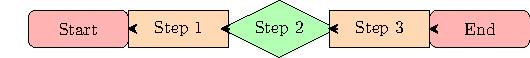
\includegraphics{figures/methodology}
  \caption{Overview of our methodology}
  \Description{This figure provides an overview of the methodology that we took for this paper}
  \label{fig:approach}
\end{figure*}

\section{Results}
\label{sec:results}


\section{Discussion}
\label{sec:discussion}

\section{Threats to Validity}
\label{sec:threats_to_validity}

\section{Conclusion}
\label{sec:conclusion}

%\section*{Acknowledgments}
\bibliographystyle{ACM-Reference-Format}
\bibliography{paper.bib}

\end{document}

\endinput
